\chapter{Configuration Spaces}

\section{Definitions and preliminary results}
% These definitions are presented in Abrams on page 10.
Given a topological space \(X\), the \(n\) point (topological) configuration space of \(X\) is
\(\Conf_n(X) = X^n - \Delta\) where \(\Delta\) is the diagonal in \(X^n\).

Treating a graph \(\Gamma\) as a topological space we can construct the
\(n\) point discretized or combinatorial configuration space \(\DConf_n(\Gamma)\) by 
% this diagonal needs elaboration.
removing a larger diagonal \(\Delta^{\square} = \{(e_1, \ldots, e_n) \mid x_i \cap x_j \neq \emptyset \text{ for some } i \neq j\}\)
from \(\Gamma^n\). Here \((e_1, \cdots, e_n)\) is any \(n\)-tuple of cells in \(\Gamma\).

Abrams showed in \cite{abrams2000configurationspaces} that \(\Conf_n(\Gamma)\) deformation retracts onto \(\DConf_n(\Gamma)\) and
that \(\DConf_n(\Gamma)\) is a cubical complex.
He also notes that any point in the
\(n\)-point configuration space is in one-to-one correspondence with a
collection of ``tokens'' placed on the graph. In this project, we will use a slightly different terminology and
and say ``particles'' instead of ``tokens.''

% TODO what is a cubical complex?
% make sure to define n-cubes and the gluing map

\begin{figure}[h!]
\centering
\begin{tikzpicture}
    \node (u1) at (2, 2) {\(u_1\)};
    \node (u2) at (4, 2) {\(u_2\)};
    \node (u3) at (3, 1) {\(u_3\)};
    \node (u4) at (3, 0) {\(u_4\)};
    \draw (u1) -- (u3);
    \draw (u2) -- (u3);
    \draw (u4) -- (u3);
\end{tikzpicture}
\caption{The \(Y\)-graph}
\label{fig:ygraph}
\end{figure}
Imagine \(2\) particles placed on the graph in \ref{fig:ygraph} at \(u_1\) and \(u_2\).  
In the topological configuration space, as the particle at \(u_1\) moves to \(u_3\)
the particle at \(u_2\) is free to simultaneously move to \(u_3\) as well. 
However, both particles would not be able to occupy the vertex \(u_3\) simultaneously.  
Compare this with the combinatorial configuration space, as the
particle at \(u_1\) moves to \(u_3\), the particle at \(u_2\) can not move at
all since the edges \(u_1 u_3\) and \(u_2 u_3\) intersect at \(u_3\) and points
with coordinates belonging to both edges are removed.

\begin{figure}[h!]
\centering
\begin{tikzpicture}
    \node (v1) at (0, 2) {\(v_1\)};
    \node (v2) at (0, 0) {\(v_2\)};
    \draw (v1) -- (v2);
    \node (u1) at (2, 2) {\(u_1\)};
    \node (u2) at (4, 2) {\(u_2\)};
    \node (u3) at (3, 1) {\(u_3\)};
    \node (u4) at (3, 0) {\(u_4\)};
    \draw (u1) -- (u3);
    \draw (u2) -- (u3);
    \draw (u4) -- (u3);
\end{tikzpicture}
\caption{An edge and a \(Y\)-graph}
\label{fig:edgeygraph}
\end{figure}
Now consider the graph in figure \ref{fig:edgeygraph} and put particles at \(v_1\) and \(u_3\).
As the particle at \(v_1\) moves to \(v_2\) there are three ways that the particle at \(u_3\) can move.
Since each way that the particle at \(u_3\) can move can be done simultaneously as the movement of the particle at \(v_1\),
the \(1\)-cell corresponding to the movement of the particle at \(v_1\) to \(v_2\)
borders three distinct \(2\)-cubes (see figure \ref{fig:threepagebook}).
We call this structure a \(3\)-page book.

\begin{figure}[h!]
\centering
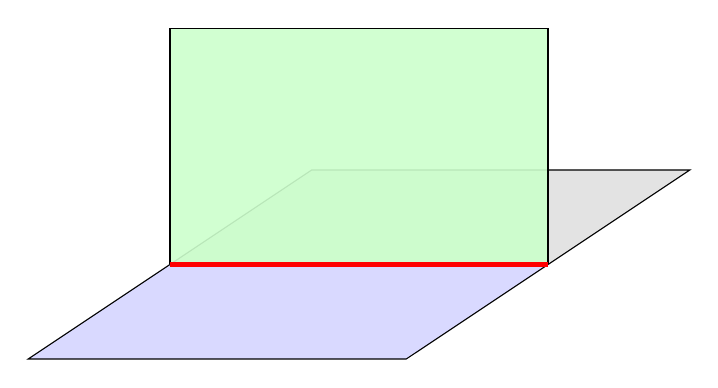
\begin{tikzpicture}[
    scale=1.2,
    % Define a 3D-like perspective by setting the coordinate vectors.
    % x goes to the right, y goes up, and z gives a sense of depth.
    z={(-0.6cm,-0.4cm)}, 
    x={(1cm,0cm)},      
    y={(0cm,1cm)}       
]
    % --- Define Coordinates for the vertices of the book ---
    
    % The spine is a 1-cell from O to A
    \coordinate (O) at (0,0,0);
    \coordinate (A) at (4,0,0);

    \coordinate (B_Back) at (4,0,-2.5);
    \coordinate (C_Back) at (0,0,-2.5);

    \coordinate (B_Front) at (4,0,2.5);
    \coordinate (C_Front) at (0,0,2.5);

    \coordinate (B_Up) at (4,2.5,0);
    \coordinate (C_Up) at (0,2.5,0);

    % Draw book pages
    \fill[gray!30, opacity=0.75] (O) -- (A) -- (B_Back) -- (C_Back) -- cycle;
    \draw (O) -- (C_Back) -- (B_Back) -- (A);

    \fill[blue!20, opacity=0.75] (O) -- (A) -- (B_Front) -- (C_Front) -- cycle;
    \draw (O) -- (C_Front) -- (B_Front) -- (A);

    \fill[green!20, opacity=0.9] (O) -- (A) -- (B_Up) -- (C_Up) -- cycle;
    \draw (O) -- (C_Up) -- (B_Up) -- (A);

    % --- Draw the Spine on top so it stands out ---
    \draw[line width=1.5pt, red] (O) -- (A);
\end{tikzpicture}
\caption{A 3-page book}
\label{fig:threepagebook}
\end{figure}

% It would make so much more sense if we excluded the covers of the book when counting the pages.
% Then, a book with more than 0 pages is not homeomorphic to a surface. 
% However, this would be an annoying substitution in later proofs.
\begin{defn}
    An \(n\)-page book is a collection of \(n\) \(2\)-cubes each glued along a common edge.
    This edge is called the spine of the book.
\end{defn}

Books are common structures found in configuration spaces.
One goal for this project is to determine which configuration spaces are surfaces.

\begin{thm}
A book with more than \(2\) pages is not a surface.
\end{thm}
\begin{proof}
Suppose there exists an \(n\)-page book that is a surface but \(n > 2\).
Let \(p\) be some point in the interior of the book's spine.
% pg. 225 Munkres states that an m-manifold X is a Hausdorff space such that for each point x in 
% X there exists a nehiborhood of x that is homeomorphic to an open subset of R^m.
% Let U be the neihborhood of p in X, V be the open subset of R^2, and \phi
% be the homeomorphism from U to V.
% Take some open disk B centered at \phi(p) in V such that \closure{B} \subseteq V
% restrict \phi to this open disk (this is okay to do in the codomain as \phi is a bijection).
Since the book is homeomorphic to a surface, there exists an open neighborhood \(U\) of \(p\)
which is homeomorphic to an open disk \(B\) in \(\mathbb{R}^2\).
Let \(\phi\) be a homeomorphism from \(\closure{U}\) to \(\closure{B}\) and \(S\) be the portion of book's spine inside of \(U\).
Notice that \(U \setminus S\) consists of \(n\) path components--one from each page of the book.
However,
\[
U\setminus S \cong \phi(U\setminus S) = B \setminus \phi(S).
\]

We claim that \(\phi(S)\) must separate \(B\) into two components.
To see this, first note that \(\phi(S)\) is a properly imbedded arc in \(B\) with \(\Bd(\phi(S))\) consisting of two
points on \(\Bd(B)\).
% homemorphisms map boundary points to boundary points, interior points to interior points, and exterior points to exterior points.
% This is common knowledge but a proof might be necessary TODO.
Since \(\Bd(B)\) is homeomorphic to a circle, there exists two different paths \(\alpha\) and \(\beta\) 
connecting these two points together (See Figure \ref{fig:thm:book_1_1}).

\begin{figure}[h!]
    \centering
    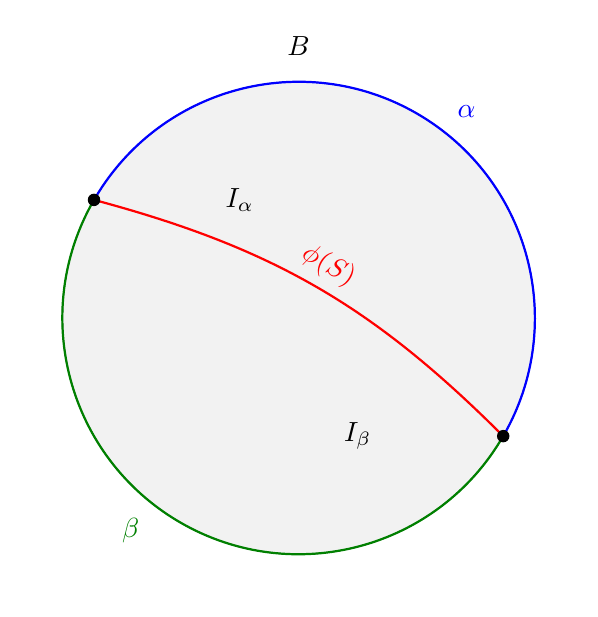
\begin{tikzpicture}[scale=1.5]
        % Define the main circle (the disk D^2) and fill it lightly
        \fill[gray!10] (0,0) circle (2cm);
        \draw (0,0) circle (2cm);
        \node at (0, 2.3) {\(B\)};

        % Define the start and end points of the arc on the boundary of the disk
        \coordinate (P1) at (150:2cm);
        \coordinate (P2) at (-30:2cm);

        % Draw the separating arc phi(S \cap U) with a distinct color
        \draw[thick, red] (P1) to[bend left=15] node[above, pos=0.5, sloped] {\(\phi(S)\)} (P2);

        % Draw the boundary path alpha
        \draw[thick, blue] (P2) arc (-30:150:2cm);
        \node[blue, above, xshift=18pt, yshift=-5pt] at (60:2cm) {\(\alpha\)};
        
        % Draw the boundary path beta
        \draw[thick, green!50!black] (P1) arc (150:330:2cm);
        \node[green!50!black, below, xshift=-18pt, yshift=5pt] at (240:2cm) {\(\beta\)};
        
        % Label the two regions separated by the arc
        \node at (-0.5, 1) {\(I_{\alpha}\)};
        \node at (0.5, -1) {\(I_{\beta}\)};
        
        % Mark the endpoints on the boundary
        \fill (P1) circle (1.5pt);
        \fill (P2) circle (1.5pt);

    \end{tikzpicture}
    \caption{The arc \(\phi(S)\) separates the open disk \(B\) into two components, \(I_{\alpha}\) and \(I_{\beta}\).}
    \label{fig:thm:book_1_1}
\end{figure}

The Jordan curve theorem guarantees that the simple closed curve \(\alpha \cup \phi(S)\) (resp. \(\beta \cup \phi(S)\))
separate \(B \setminus (\alpha \cup \phi(S))\) (resp. \(B \setminus (\beta \cup \phi(S))\)) into a bounded connected component
\(I_{\alpha}\) and an unbounded connected component \(O_{\alpha}\) (resp. \(I_{\beta}\) and \(O_{\beta}\)) when imbedded in \(\mathbb{R}^2\).
Notice \(B\setminus \phi(S) = I_{\alpha} \cup I_{\beta}\).
Since \(I_{\alpha} \subseteq O_{\beta}\) and \(I_{\beta} \cap O_{\beta} = \emptyset\),
we have that \(I_{\alpha} \cap I_{\beta} = \emptyset\).
So, \(I_{\alpha}\) and \(I_{\beta}\) form a separation of \(B\setminus \phi(S)\).
\end{proof}

Another common structure found found in graph configuration spaces are \(n\)-cubes.
Consider the graph in Figure \ref{fig:3edges} and imagine \(3\) particles placed at \(u_1\), \(v_1\), and \(w_1\).
Each particle can simultaneously move to \(u_2\), \(v_2\), and \(w_2\) resulting in \(3\)-cube in the configuration space (see Figure \ref{fig:3cube}).

\begin{figure}[h!]
    \centering
\begin{tikzpicture}
    \node (u1) at (0, 2) {\(u_1\)};
    \node (u2) at (0, 0) {\(u_2\)};
    \draw (u1) -- (u2);
    \node (v1) at (2, 2) {\(v_1\)};
    \node (v2) at (2, 0) {\(v_2\)};
    \draw (v1) -- (v2);
    \node (w1) at (4, 2) {\(w_1\)};
    \node (w2) at (4, 0) {\(w_2\)};
    \draw (w1) -- (w2);
\end{tikzpicture}
    \caption{Three edges}
    \label{fig:3edges}
\end{figure}

\begin{figure}[h!]
    \centering
    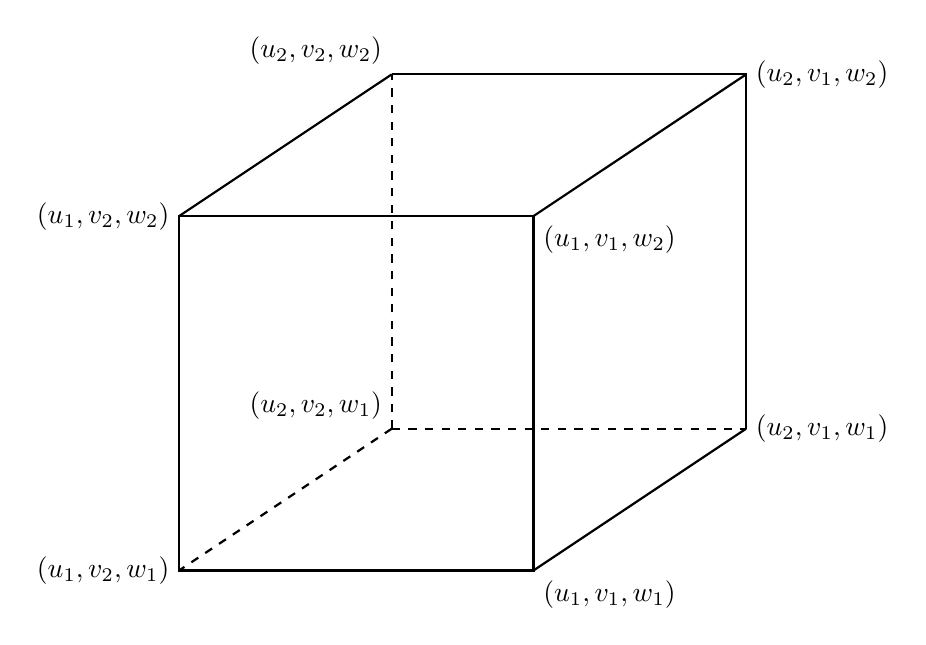
\begin{tikzpicture}[
    scale=1.5,
    % Define a 3D-like perspective by setting the coordinate vectors.
    % x goes to the right, y goes up, and z gives a sense of depth.
    x={(1cm,0cm)},
    y={(0cm,1cm)},
    z={(-0.6cm,-0.4cm)}
]
    % --- Style Definitions ---
    % Define styles for the cube's edges to make the code cleaner.
    % 'visible' edges are solid and thick.
    % 'hidden' edges are dashed and thick.
    \tikzstyle{visible} = [draw, thick, black]
    \tikzstyle{hidden} = [draw, thick, dashed, black]

    % --- Vertex Coordinates ---
    % Define the 8 vertices of the cube using (x,y,z) coordinates.
    % The side length of the cube is 3 units.
    \def\s{3}
    \coordinate (A) at (0,0,0);
    \coordinate (B) at (\s,0,0);
    \coordinate (C) at (\s,\s,0);
    \coordinate (D) at (0,\s,0);
    \coordinate (E) at (0,0,\s);
    \coordinate (F) at (\s,0,\s);
    \coordinate (G) at (\s,\s,\s);
    \coordinate (H) at (0,\s,\s);

    % --- Draw Hidden Edges ---
    % Draw the edges that would be obscured from view first. These are the
    % edges connected to the rearmost vertex (A).
    \draw[hidden] (A) -- (B);
    \draw[hidden] (A) -- (D);
    \draw[hidden] (A) -- (E);

    % --- Draw Visible Edges ---
    % Draw the visible edges on top of the hidden ones.
    \draw[visible] (B) -- (C) -- (D);
    \draw[visible] (E) -- (F) -- (G) -- (H) -- cycle;
    \draw[visible] (B) -- (F);
    \draw[visible] (C) -- (G);
    \draw[visible] (D) -- (H);

    % --- Optional: Label Vertices ---
    % Uncomment the following lines to add labels to each vertex.
    \node at (A) [above left] {\((u_2, v_2, w_1)\)};
    \node at (B) [right] {\((u_2, v_1, w_1)\)};
    \node at (C) [right] {\((u_2, v_1, w_2)\)};
    \node at (D) [above left] {\((u_2, v_2, w_2)\)};
    \node at (E) [left] {\((u_1, v_2, w_1)\)};
    \node at (F) [below right] {\((u_1, v_1, w_1)\)};
    \node at (G) [below right] {\((u_1, v_1, w_2)\)};
    \node at (H) [left] {\((u_1, v_2, w_2)\)};    
\end{tikzpicture}
\caption{3-cube}
\label{fig:3cube}
\end{figure}

Visually \(n\)-cubes are ``clearly'' not surfaces when \(n > 2\).
However, we can show this formally with an argument using the fundamental group.
\begin{thm}
\(n\)-cubes are not surfaces when \(n > 2\).
\end{thm}
\begin{proof}
    Suppose an \(n\)-cube \(C\) is a surface for some \(n > 2\).
    % imbed C in R^n
    Pick some point \(p\) in the interior of \(C\).
    Since \(C\) is a surface there exists some open ball \(B^n(p, \epsilon)\) in the interior of \(C\) such that 
    it is centered at \(p\) and is homeomorphic to some open neighborhood \(V\) of \(\mathbb{R}^2\).
    Let \(q\) be the point in \(V\) corresponding to \(p\).
    
    % TODO just use the fact that local simple connectedness fails after removing a point in D^2 but doesn't after removing a point in S^2.
\end{proof}

Books and cubes are the meat and potatos of the coming proofs.

\section{Computing the Euler characteristic of graph configuration spaces}
To compute the euler characteristic of an unorderd \(n\) point graph configuration space we need to count
for each \(0 \le k \le n\) the number of \(k\)-cubes present.
Without further mention \(E = E(\Gamma)\) and \(V = V(\Gamma)\).

A \(k\) cube exists if and only if \(k\) particles are free to move simultaneously while \(n - k\)
particles remain fixed.
Hence the general formula for the number of \(k\) cubes in \(\DUConf_n(\Gamma)\) is
\[
    \abs{\phi(k)} \cdot \begin{pmatrix}\abs{V} - 2k \\ n - k\end{pmatrix}
\]
where \(\phi(k)\) defined as follows.

\begin{defn}
\(\phi(k)\) is the collection consisting of all unordered sets of exactly \(k\) disjoint edges in \(\Gamma\)
where \(\phi(0) = \{\emptyset\}\).
\end{defn}

Note that we define \(\phi(0) = \{\emptyset\}\) so that \(\abs{\phi(0)} = 1\).
With this definition, \(\abs{\phi(k)}\) is also known as the number of ``\(k\)-matchings'' in \(\Gamma\).

Counting the number of \(k\)-matchings for small graphs can be done efficiently 
with a simple sweep over all \(k\) combinations of edges.
However, for general larger graphs this computation quickly becomes unwieldly.

% TODO read/cite Mark Jerrum's paper "Two-dimensional monomer-dimer systems are computationally intractable"
% where he proves computing the matching polynomial for planar graphs is P# ?
% TODO: reference program actually used to make computations? It's trivial especially now with AI hah

\begin{figure}[h!]
\centering
\begin{tabular}{c | c | c}
   \(\Gamma\) & \(n\) & \(\chi(\DUConf_n(\Gamma))\) \\
   \hline
   \(K_5\) & 2 & -5 \\
   \(K_{3,3}\) & 2 & -3 \\
   \(K_5\) & 3 & -5 \\
   \(\Theta_4\) & 3 & -4 \\
   \(K_{3,3}\) & 4 & -3
\end{tabular}
\label{fig:euler_characteristics}
\caption{Euler characteristic of certain unordered graph configuration spaces.}
\end{figure}

A workaround for this computational challenge is determing the Euler characteristic of certain classes of graphs.
In \cite{appiah2024algebraicstructurehyperbolicgraph} the ``pulsar'' graph was defined.


\begin{figure}[h!]
    \centering
\begin{tikzpicture}[scale=1]
    % Define the two main suspension vertices, positioned closer together
    \node (a1) at (0, 1) {\(a_1\)};
    \node (a2) at (0, -1) {\(a_2\)};

    % Define the intermediate vertices for the 'm' paths
    \node (b1) at (-1, 0) {\(b_1\)};
    \node (bm) at (1, 0) {\(b_m\)};
    \node at (0,0) {\(\dots\)};

    % Draw the edges for the 'm' paths, passing through the b_i nodes
    \draw (a1) to[out=180, in=90] (b1);
    \draw (b1) to[out=270, in=180] (a2);

    \draw (a1) to[out=0, in=90] (bm);
    \draw (bm) to[out=270, in=0] (a2);

    % Define vertices for the 'n1' rays attached to a1, spread out as in the drawing
    \node (c1) at (-1, 2) {\(c_1\)};
    \node (c1p) at (-2, 3) {\(c'_1\)};
    \node (cn1) at (1, 2) {\(c_{n_1}\)};
    \node (cn1p) at (2, 3) {\(c'_{n_1}\)};
    \node at (0, 2.5) {\(\dots\)};

    % Draw edges for the 'n1' rays
    \draw (a1) -- (c1);
    \draw (c1) -- (c1p);
    \draw (a1) -- (cn1);
    \draw (cn1) -- (cn1p);

    % Define vertices for the 'n2' rays attached to a2, also spread out
    \node (d1) at (-1, -2) {\(d_1\)};
    \node (d1p) at (-2, -3) {\(d'_1\)};
    \node (dn2) at (1, -2) {\(d_{n_2}\)};
    \node (dn2p) at (2, -3) {\(d'_{n_2}\)};
    \node at (0, -2.5) {\(\dots\)};

    % Draw edges for the 'n2' rays
    \draw (a2) -- (d1);
    \draw (d1) -- (d1p);
    \draw (a2) -- (dn2);
    \draw (dn2) -- (dn2p);
\end{tikzpicture}
\label{fig:pulsargraph}
\caption{The Pulsar graph \(\mathcal{P}_{m,n_1,n_2}\)}
\end{figure}

\begin{thm}
    \label{thm:pulsargrapheuler}
    The Euler characteristic of \(\DUConf_{3}(\mathcal{P}_{m,n_1,n_2})\) is
    \[
    \frac{m^{3}}{6} - \frac{3 m^{2}}{2} - \frac{m n_{1}^{2}}{2} - \frac{3 m n_{1}}{2} - \frac{m n_{2}^{2}}{2} - \frac{3 m n_{2}}{2} + \frac{7 m}{3} - \frac{n_{1}^{3}}{3} + \frac{7 n_{1}}{3} - \frac{n_{2}^{3}}{3} + \frac{7 n_{2}}{3}.
    \]
\end{thm}
\begin{proof}
%TODO: all we really have to do is explain the argument for the 2 and 3 matchings.
\end{proof}

\begin{rem}
Substituting in \(n_1 = 0\) and \(n_2 = 0\) the pular graph becomes \(\Theta_m\).
So, 
the euler characteristic of \(\DUConf_3(\Theta_m)\) is
\[
\frac{m^{3}}{6} - \frac{3 m^{2}}{2} + \frac{7 m}{3}
\]
This aligns with results in section 4 of \cite{appiah2024algebraicstructurehyperbolicgraph}.
\end{rem}